\chapter{ArcFace}\label{ch:arcface}
ArcFace~\cite{ArcFace} is a research which became public in 2018 and achieved state-of-the-art results on LFW dataset.

ArcLoss is based on the equation of \textit{softmax loss}~\ref{eq:softmax}.
There are few steps separating the original and the improved version:
\begin{enumerate}
    \item First step is to fix the bias $b_j = 0$.
    \item Then we transform the logit as $W_j^T x_i = \norm{W_j} \norm{x_j} cos \theta_j$
    $\theta$ is the angle between the weight $W_j$ and the feature $x_i$.
    \item In a third step we fix the individual weights $\norm{W_j} = 1$ by $l_2$ normalization
    \item We do the same for feature $x_i$ and re-scale it to $s$ where coefficient $s$ is predetermined feature scale.
    These normalization steps make the prediction depend only on the angle $\theta$.
    The embeddings are distributed on the hypersphere with a radius $s$.
\end{enumerate}

\begin{figure}[H]
    \centering
    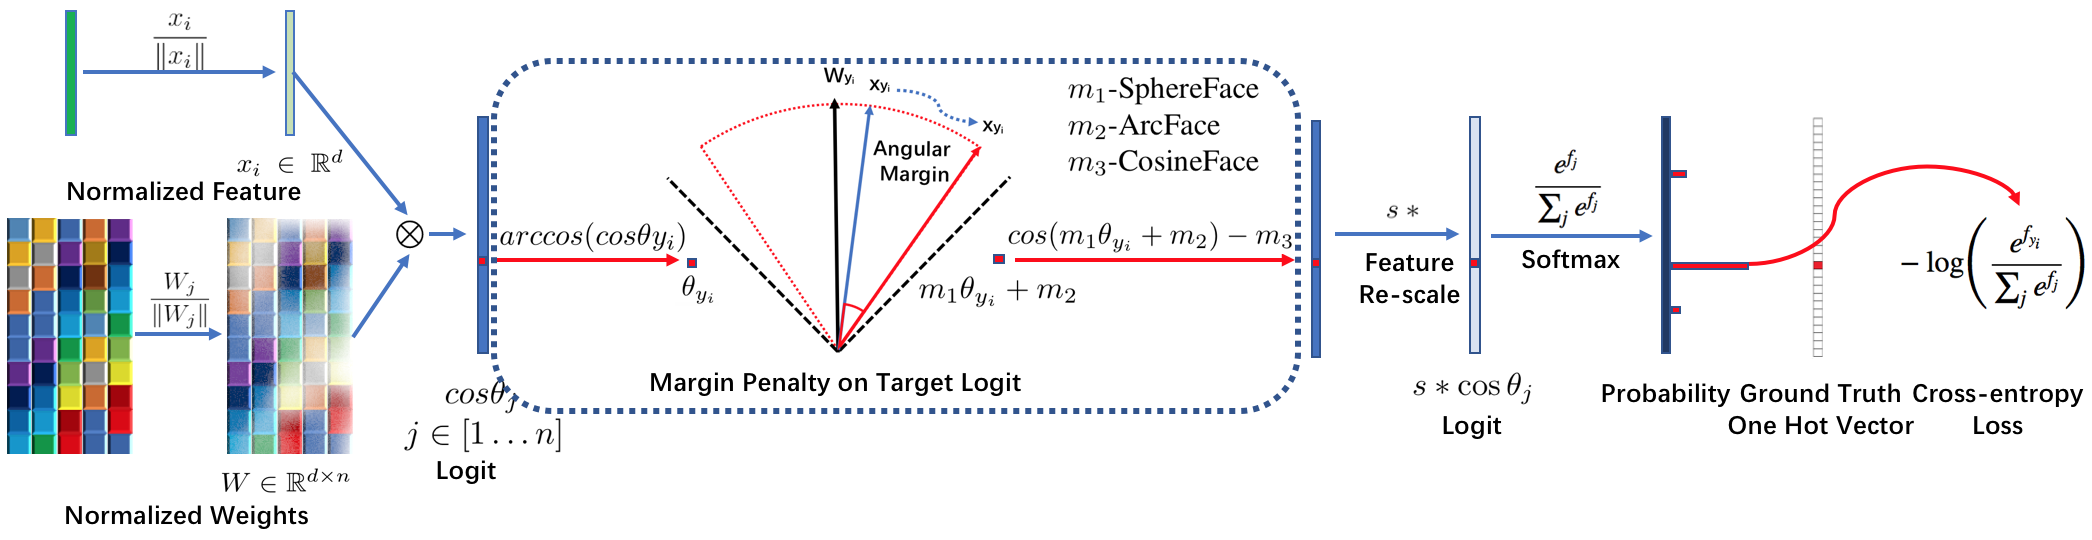
\includegraphics[width=\columnwidth]{images/arcface/arcface.png}
    \caption{Training a CNN for face recognition supervised by the ArcFace loss~\cite{ArcFace}}
    \label{fig:arcface}
\end{figure}